\documentclass[tikz, border=5mm]{standalone}
\usepackage{textcomp}
\usetikzlibrary{arrows.meta,decorations.markings,fit,calc, positioning}

\definecolor{componentColor}{RGB}{210,210,210}
\definecolor{systemColor}{RGB}{230,230,230}

\tikzset{component/.append style={fill=componentColor, align=center, draw, minimum width=2cm, minimum height=1.5cm, rounded corners=.3cm}}
\tikzset{system/.style={ component, fill=systemColor, rounded corners=0cm}}


\begin{document}

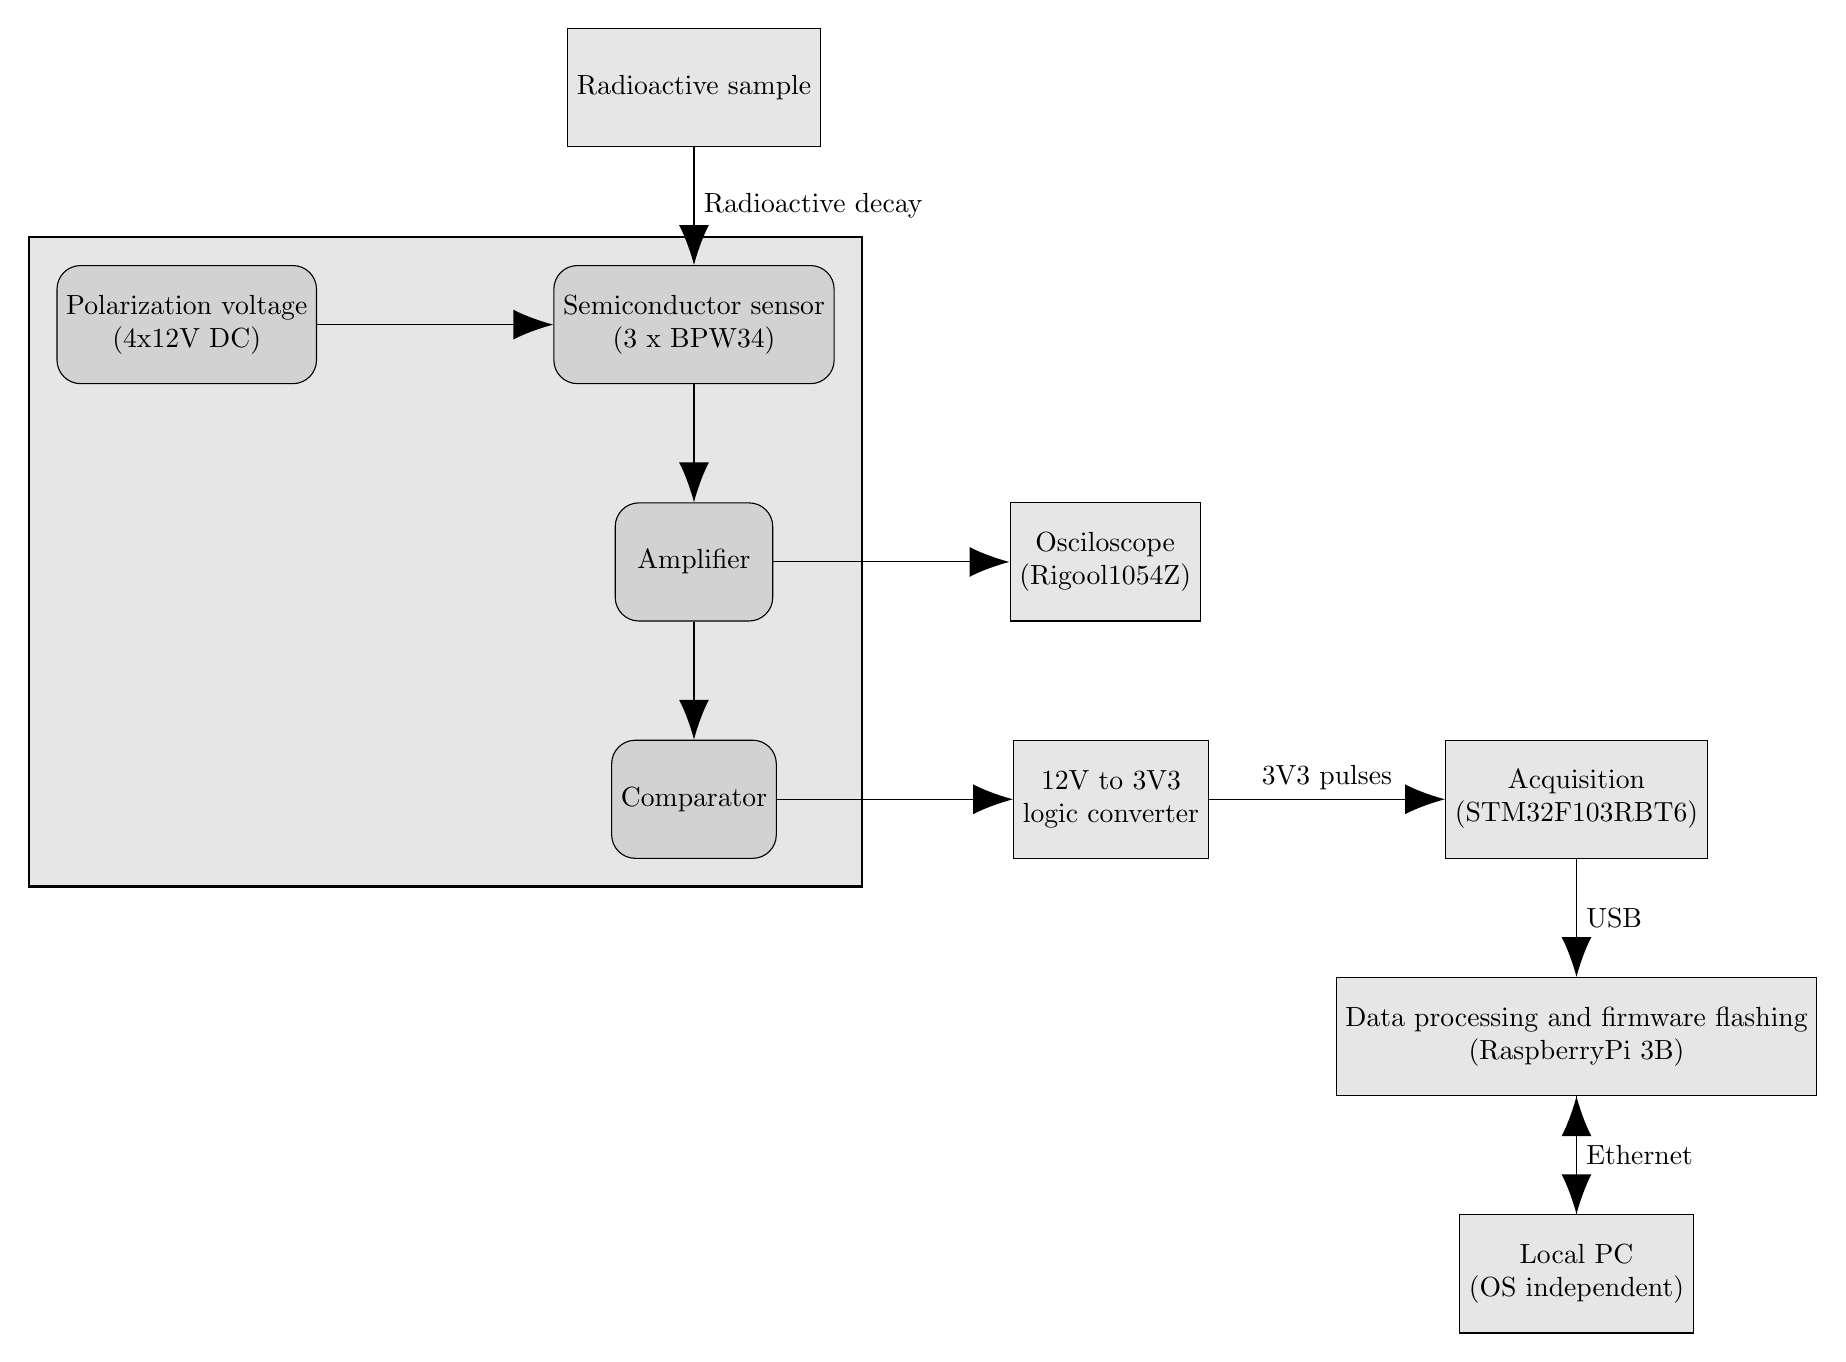
\begin{tikzpicture}[node distance=1.5cm and 3cm]
% Nodes
\pgfdeclarelayer{background}
\pgfsetlayers{background,main}

\node (chamber) [component] {Semiconductor sensor\\ (3 x BPW34)};
\node (sample) [system, above=of chamber] {Radioactive sample};

\node (polarization) [component, left=of chamber] {Polarization voltage\\ (4x12V DC)};
\node (amplifier) [component, below=of chamber] {Amplifier};

\node (osciloscope) [system, right=of amplifier] {Osciloscope\\ (Rigool1054Z)};

\node (comparator) [component, below=of amplifier] {Comparator};
\node (converter) [system, right=of comparator] {12V to 3V3\\ logic converter};

\node (cpu) [system, right=of converter] {Acquisition\\ (STM32F103RBT6)};

\node (pi) [system, below=of cpu] {Data processing and firmware flashing\\ (RaspberryPi 3B)};
\node (pc) [system, below=of pi] {Local PC\\ (OS independent)};


\begin{pgfonlayer}{background}
\node[system ,  draw, thick,  inner xsep=1em, inner ysep=1em, fit=(chamber) (polarization) (amplifier) (comparator) ] {};
\end{pgfonlayer}

% Connectors
\begin{scope}[->]

\draw [-{Latex[scale=3.0]}] (sample) -- node[anchor=west, minimum width=.25cm, draw=none] {Radioactive decay} (chamber);
\draw [-{Latex[scale=3.0]}] (polarization) -- node[anchor=south, minimum width=.25cm, draw=none] {} (chamber);
\draw [-{Latex[scale=3.0]}] (chamber) -- node[anchor=south, minimum height=.25cm, draw=none] {} (amplifier);
\draw [-{Latex[scale=3.0]}] (amplifier) -- node[anchor=south, minimum height=.25cm, draw=none] {} (osciloscope);

\draw [-{Latex[scale=3.0]}] (amplifier) -- node[anchor=south, minimum height=.25cm, draw=none] {} (comparator);
\draw [-{Latex[scale=3.0]}] (comparator) -- node[anchor=south, minimum height=.25cm, draw=none] {} (converter);
\draw [-{Latex[scale=3.0]}] (converter) -- node[anchor=south, minimum height=.25cm, draw=none] {3V3 pulses} (cpu);
\draw [-{Latex[scale=3.0]}] (cpu) -- node[anchor=west, minimum height=.25cm, draw=none] {USB} (pi);

\draw [-{Latex[scale=3.0]}] (pi) -- node[anchor=west, minimum height=.25cm, draw=none] {Ethernet} (pc);
\draw [-{Latex[scale=3.0]}] (pc) -- node[anchor=west, minimum height=.25cm, draw=none] {} (pi);

\end{scope}

\end{tikzpicture}
\end{document}
